\documentclass{beamer}
\input{../style/cours-style.sty}

% Title
\title[JavaScript]{JavaScript Frontend - B1 Web et Multimédia}
\author{Christophe Brun}
\institute{My Digital School}
\beamertemplatenavigationsymbolsempty

\titlegraphic{
    \bigbreak
    
\includegraphics[width=5cm]{image/mds-logo}
    \bigbreak
    L’école des métiers du digital
    \bigbreak
}

\begin{document}

    \begin{frame}
        \titlepage
        \bigbreak
        \centering
        \url{https://github.com/My-Digital-School-by-PapIT/frontend-JS}
    \end{frame}


    \section{Table des matières}\label{sec:toc}

    \begin{frame}{Table des matières}
        \begin{tiny}
            \begin{multicols}{1}
                \tableofcontents
            \end{multicols}
        \end{tiny}
    \end{frame}


    \section{Programme du module}\label{sec:programme-du-module}

    \begin{frame}{JavaScript Frontend}{Objectifs des 6 jours}
        \begin{columns}
            \column{0.7\textwidth}
            \begin{scriptsize}
                \begin{itemize}
                    \item Distinguer les différentes parties prenantes du web (protocol de communication, navigateur, serveur, \textit{etc}).
                    \item La syntaxe JavaScript.
                    \item La Window API, manipulation de DOM.
                    \item Intéragir avec une API depuis le frontend.
                \end{itemize}
            \end{scriptsize}
            \column{0.3\textwidth}
            
\includegraphics[width=4cm]{image/js-surfing}
        \end{columns}
    \end{frame}


    \section{Introduction}\label{sec:introduction}

    \begin{frame}{Formateur sur Linux}{Christophe Brun, conseil en développement informatique}

        \begin{columns}
            \column{0.7\textwidth}
            \begin{itemize}
                \item Développeur freelance (Python, Java, CoBOL) et data at scale.

                \item 7 ans de conseil en développement au sein d'SSII~.

                \item 7 ans de conseil en développement en indépendant, \href{https://papit.fr}{PapIT}.

                \item Passionné~!
                \bigbreak
                \begin{columns}
                    \column{0.5\textwidth}
                    \centering
                    
\includegraphics[width=3cm]{image/logo-uppa}
                    \column{0.5\textwidth}
                    \centering
                    
\includegraphics[width=3cm]{image/logo-universite-bordeaux}
                \end{columns}
            \end{itemize}
            \column{0.3\textwidth}
            \centering
            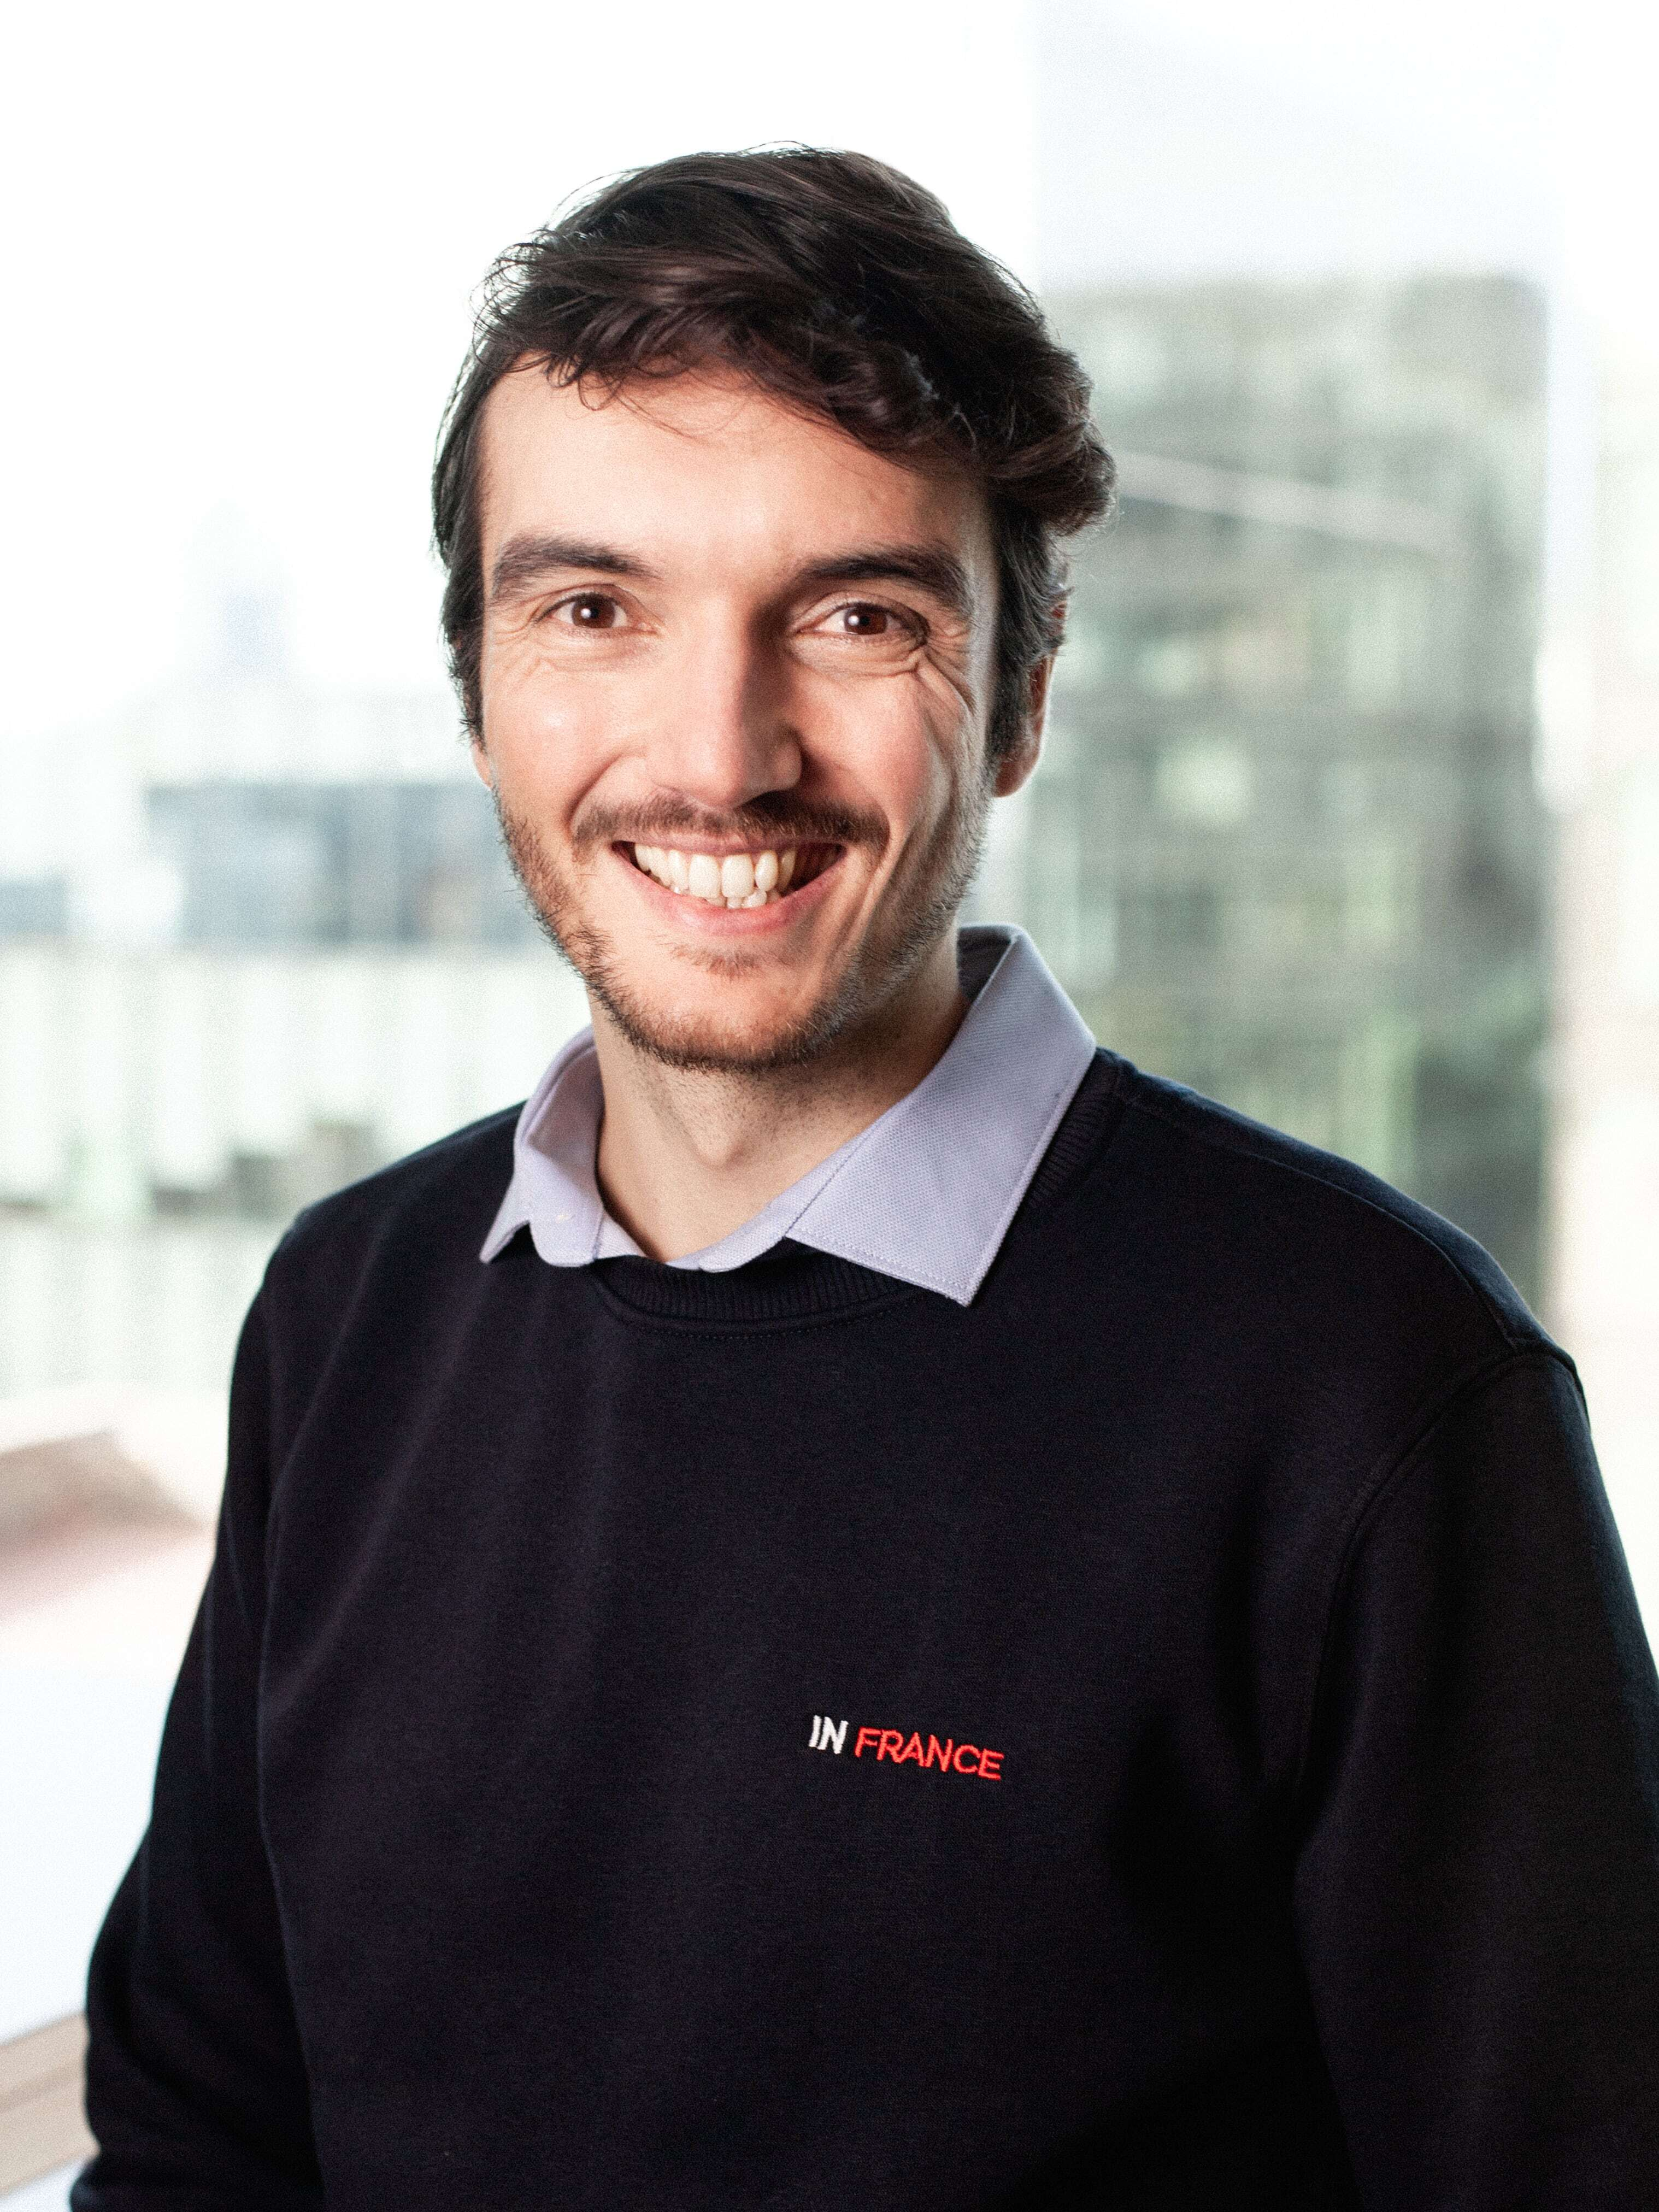
\includegraphics[width=5cm]{image/trombine-christophe}
        \end{columns}
    \end{frame}


    \section{Les ressources du Web}\label{sec:ressources}

    \begin{frame}{Les ressources du Web}{Dvisions en briques}
        \begin{columns}
            \column{0.6\textwidth}
            1 des 4 règles pour la direction de l'esprit de Descartes~: \textquote{Diviser chacune des difficultés que j'examinerais, en autant de parcelles qu'il se pourrait et qu'il serait requis pour les mieux résoudre.}.
            \column{0.4\textwidth}
            \centering
            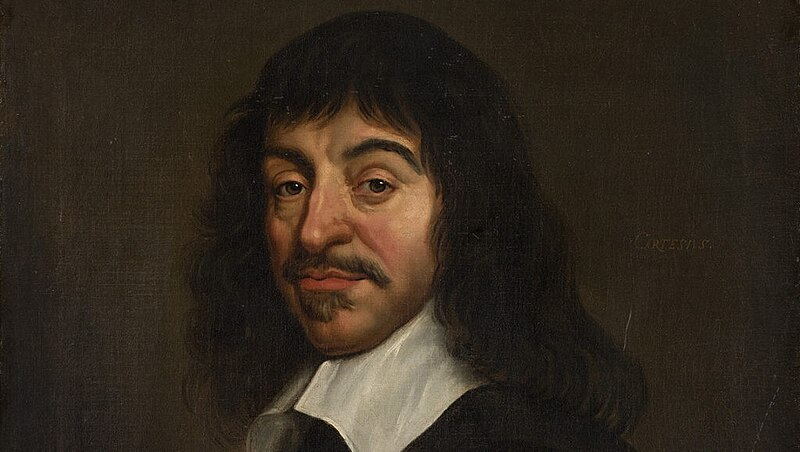
\includegraphics[width=6cm]{image/Descartes}
        \end{columns}
    \end{frame}

    \begin{frame}{Les ressources du Web}{Analyse des composants}
        \centering
        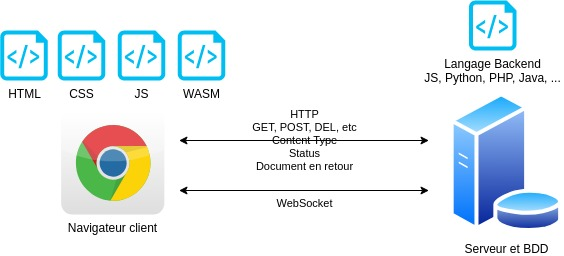
\includegraphics[width=11cm]{image/web-stakeholders.drawio}
    \end{frame}


    \section{Le web statique}\label{sec:static}

    \begin{frame}{Le web statique}
        Une des premières options pour un site web est donc d'être statique.

        Suite à une requête sur une URL (adresse dans le navigateur), le serveur nous envoie une page HTML pour la donnée avec du CSS pour le style.
        \bigbreak
        Il n'y a pas d'interaction avec le serveur, le contenu est figé, on peut juste passer à une autre page grâce à une ancre \lstinline{<a href="...">...</a>}.
        \bigbreak
        \centering
        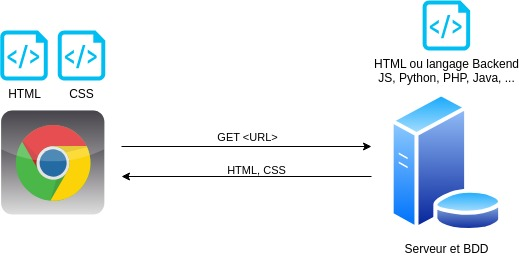
\includegraphics[width=8cm]{image/web-static}
    \end{frame}

    \begin{frame}[fragile]{Développement Web Statique}{Exercice \execcounterdispinc{}}
        \begin{itemize}
            \item Installer Python 3.
            \item Installer un IDE de développement Web comme WebStorm.
            \item Lancer un serveur HTTP avec la commande dans le répertoire du cours~:
            \begin{lstlisting}[language=bash]
python3 -m http.server
            \end{lstlisting}
            \item Naviguer à l'adresse indiquée.
            \item Modifier le fichier \lstinline{index.html} pour ajouter un lien vers une page HTML développée par vos soins avec votre nom et une photo de vous.
            \item Rafraîchir la page et vérifier que la modification est fonctionnelle.
        \end{itemize}
    \end{frame}


    \section{Le web dynamique}\label{sec:Dynamic}
    \begin{frame}{Développement Web Dynamique}{Exercice \execcounterdispinc{}}
        \begin{itemize}
            \item Quelles seraient les moyens d'avoir des pages web dynamiques~?
        \end{itemize}
        \bigbreak
        \centering
        
\includegraphics[width=5cm]{image/question-mark}
    \end{frame}

    \begin{frame}{Développement Web Dynamique}{Backend}
        Un serveur qui fait tourner un algorithme qui sert des données qui évoluent (dans la base de données), ou de l'extérieur (API).

        Plusieurs requêtes sont nécessaires, de différents types~:
        \begin{itemize}
            \item Des GET comme auparavant pour retourner des données.
            \item Des POST pour envoyer des données au serveur.
            \item Des DEL pour supprimer des données de la base de données du serveur.
        \end{itemize}
        \bigbreak
        \centering
        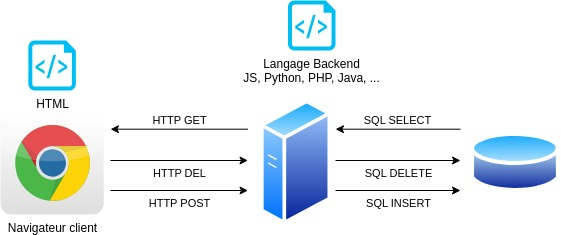
\includegraphics[width=7cm]{image/web-dynamic-backend}
    \end{frame}

    \begin{frame}{Frontend}
        \begin{small}
            Il est également possible de modifier une page web sans recharger la page entière, en utilisant JavaScript.

            Le JavaScript est un des langages qui peuvent être interprétés par le navigateur.

            Ces langages sont~:
            \begin{itemize}
                \item \textbf{HTML}, un langage de balisage, à l'image du XML, c'est le document principal de la page.
                Il peut contenir de la mise en forme, des données à afficher, \textit{etc}.
                \item \textbf{CSS}, un langage de style, qui permet de définir la mise en forme de la page.
                C'est une manière \textbf{modulaire} de définir le style de tout un site web.
                \item \textbf{JavaScript}, un langage de programmation qui permet de modifier le contenu de la page sans recharger la page.
                Il peut modifier~:
                \begin{itemize}
                    \item Le contenu de la page, ses données (DOM API\footnotemark{}).
                    \item Le style de la page, la mise en forme (DOM API\cref{DOM}).
                    \item Intéragir avec n'importe quel serveur.
                \end{itemize}
            \end{itemize}
        \end{small}
        \footnotetext{\label{DOM}DOM (Document Object Model), \url{https://developer.mozilla.org/fr/docs/Glossary/DOM}}
    \end{frame}


    \section{Généralité sur le JavaScript en Frontend}\label{sec:js-basic}

    \begin{frame}{Où se trouve le JavaScript ?}
        Deux solutions, ils se trouvent~:
        \begin{itemize}
            \item Dans le fichier HTML, entre les balises \lstinline{<script>...</script>}.
            \item Dans un fichier séparé, avec l'attribut \lstinline{src} de la balise \lstinline{<script>} qui indique le chemin de ce fichier.
            Comme le fichier de style, cette méthode est plus modulaire, car ce fichier peut être partagé entre plusieurs pages.
        \end{itemize}
        \bigbreak
        \begin{dangercolorbox}
            En programmation, être modulaire est une importante qualité. Si on réutilise, on est écrit moins.
            Ici, dans un seul fichier.
            Si on écrit moins, on écrit moins de bug~!
        \end{dangercolorbox}
    \end{frame}

    \begin{frame}{Exercice \execcounterdispinc{}}
        \begin{itemize}
            \item Trouver le script javascript du fichier \lstinline{index.html}.
            \item Créer un fichier \lstinline{script.js} dans le même répertoire que \lstinline{index.html}.
            \item Copier le contenu du script dans ce fichier.
            \item Adapter le fichier \lstinline{index.html} pour inclure ce fichier en utilisant l'attribut \lstinline{src} et supprimant le contenu de la balise qui devient inutile.
            \item Simplifier la balise \lstinline{<script>} en conséquence.
            \item Rafraîchir la page et vérifier que la modification est fonctionnelle.
        \end{itemize}
    \end{frame}


    \section{Licence CC}\label{sec:licence}

    \begin{frame}{Licence}{Licence Creative Commons}
        Support de cours sous licence Creative Commons BY-NC-ND~.
        \bigbreak
        Vous pouvez donc, partager, copier, distribuer le document.
        \bigbreak
        Attribution requise à PapIT SASU - Pas d’utilisation commerciale - Pas de modification
        \bigbreak
        \centering
        
\includegraphics[width=5cm]{image/by-nc-nd-logo}
    \end{frame}


\end{document}
